\subsection{Extraktion}\label{subsec:extraction}
Im ersten Schritt werden die Videos zu einem Trainingsdatensatz verarbeitet.
\begin{lstlisting}[label={lst:extraction-1},numbers=none]
    2) extract images from video data_src.bat
    3) extract images from video data_dst FULL FPS.bat
\end{lstlisting}
Diese Skripte zerlegen mithilfe von FFmpeg das \texttt{src}- bzw. \texttt{dst}-Video in ihre einzelnen Frames.
Diese sind im \texttt{workspace} unter \texttt{data\_src} bzw. \texttt{data\_dst} zu finden.
Bei dem \texttt{src}-Video kann in der Konsole zusätzlich angegeben werden, wie viele \gls{fps} extrahiert werden sollen.
Bei langen \texttt{src}-Videos kann dies sinnvoll sein.
Werden 5 \gls{fps} aus einem 4-minütigen Video extrahiert, ist die Variation der Bilder größer als bei 10 \gls{fps} aus einem 2-minütigen Video.
Natürlich können immer auch alle Frames extrahiert werden, hier muss der größere Speicheraufwand und die längere Trainingsdauer abgewogen werden.
Da das exemplarische Video gerade einmal 655 Frames lang ist, können unbedenklich alle Frames genutzt werden.
Des Weiteren kann zwischen \texttt{PNG} und \texttt{JPG} entschieden werden.
Die Entscheidung bringt die üblichen Vor- und Nachteile der beiden Formate.
\begin{itemize}
    \item \textbf{PNG:} Verlustfreie Komprimierung \rightarrow Größere Dateien \rightarrow Kein Qualitätsverlust
    \item \textbf{JPG:} Verlustbehaftete Komprimierung \rightarrow Kleinere Dateien \rightarrow Qualitätsverlust
\end{itemize}
Da Speicherplatz für Videos dieser Länge nicht der entscheidende Faktor ist, kann hier die höhere Qualität von \texttt{PNG} genutzt werden.\\
Das \texttt{dst}-Video wird immer komplett extrahiert, da die Frames am Ende der Pipeline wieder zu einem Video zusammengesetzt werden.
Es müssen alle Frames vorhanden sein, um ein flüssiges Endergebnis zu gewährleisten.
Es kann ebenfalls das Bildformat ausgewählt werden, dieses sollte gleich gewählt werden wie beim ersten Video.

\subsubsection{Face Extraction}
Nun müssen die Gesichter aus den Bildern extrahiert werden.
Im Folgenden wird der Prozess für das \texttt{src}-Material (in \gls{dfl} Schritt 4.X) beschrieben.
Für das \texttt{dst}-Material verläuft der Prozess (als Schritt 5.X) analog.

Es gibt zwei Varianten, die Gesichter aus den Frames zu extrahieren.
\begin{lstlisting}[numbers=none,label={lst:extraction-2}]
    4) data_src faceset extract MANUAL.bat
    4) data_src faceset extract.bat
\end{lstlisting}
Wie die Namen vermuten lassen, werden die Gesichter einmal händisch und einmal durch ein vortrainiertes \gls{cnn} extrahiert.
Bei der automatischen Extraktion müssen im Nachhinein ggf. falsch erkannte Gesichter manuell gelöscht werden.
Allerdings ist dieser Arbeitsaufwand bei weitem geringer als die manuelle Extraktion.
Bei der Ausführung können verschiedene Punkte konfiguriert werden.
Der \textbf{face type} gibt an, wie viel vom Gesicht extrahiert werden soll.
\begin{itemize}
    \item \textbf{f (face):} Nur das Gesicht
    \item \textbf{wf (whole face):} Das ganze Gesicht inklusive Stirn und Kinn
    \item \textbf{h (head):} Der gesamte Kopf inklusive Haare
\end{itemize}
\textbf{Max numbers of faces} gibt an, wie viele Gesichter pro Frame extrahiert werden sollen.
Dieser Wert sollte auf 0 (alle) gesetzt werden.
Ist mehr als ein Gesicht in den Videos zu sehen, werden alle Gesichter extrahiert; nicht benötigte Bilder können anschließend wieder gelöscht werden.
Sind es zu viele Gesichter bzw. wird die Verarbeitungszeit zu hoch, muss entweder manuell oder mit einer Obergrenze extrahiert werden.
Im ersten Fall fällt erhöhter Arbeitsaufwand an, im zweiten Fall fällt der Datensatz kleiner aus, da das gewünschte Gesicht ggf. übersprungen wird.
Die Beispielvideos bestehen nur aus einem bzw. zwei Gesichtern und können unproblematisch automatisiert extrahiert werden.
Anschließend kann entweder im Standard Windows Explorer unter \texttt{workspace/data\_src/aligned} oder mithilfe des mitgelieferten Explorers die Daten gesichtet werden.
\begin{lstlisting}[label={lst:extraction-3},numbers=none]
    4.1) data_src view aligned result.bat
\end{lstlisting}
Dieses Skript öffnet den in Rust implementierten Explorer \texttt{XnView} (Abbildung \ref{fig:xnview}), welcher auf das schnelle Anzeigen von Bildern optimiert wurde.
\begin{figure}
    \center
    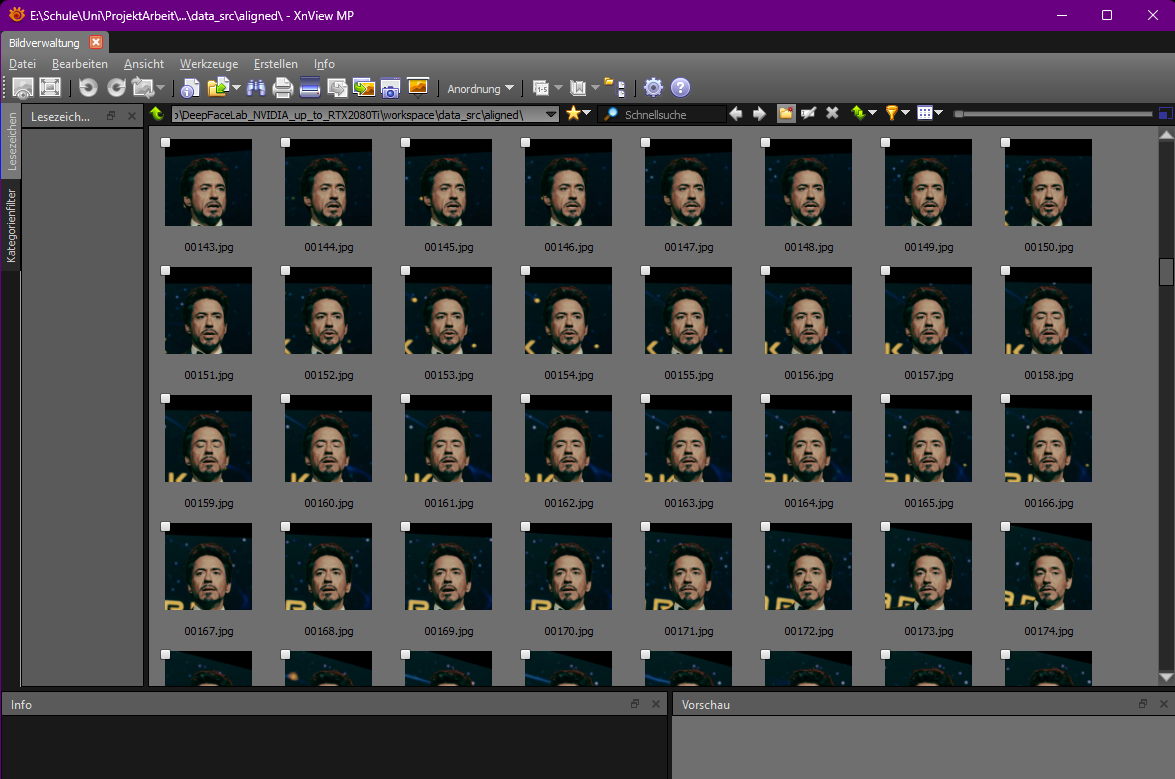
\includegraphics[width=0.7\textwidth]{Bilder/DFL/XnView}
    \caption{XnView (Rust Explorer)}
    \label{fig:xnview}
\end{figure}
Nun müssen alle Bilder, die nicht richtig erkannt wurden, gelöscht werden.
Dabei stellt \gls{dfl} einige Sortierungsmöglichkeiten zur Verfügung, die den Prozess erleichtern.
Diese sind zu einem Skript zusammengefasst.
\begin{lstlisting}[label={lst:extraction-4},numbers=none]
    4.2) data_src sort.bat
\end{lstlisting}
Durch das Sortieren nach \texttt{[0] blur} und \texttt{[1] motion\_blur} können schnell unscharfe Bilder ausfindig gemacht werden.
Durch die Sortierung nach \texttt{[5] histogram similarity} werden ähnliche Gesichter zusammen gruppiert.
So können Bilder einer nicht erwünschten zweiten Person einfach entfernt werden.\\
Ist die Auswahl der Gesichter abgeschlossen, können diese noch bei Bedarf mit \gls{ai-upscaling} vergrößert werden.
Dies sollte nur gemacht werden, wenn die Bilder sonst unscharf oder zu klein sind.
Besser ist es, direkt scharfe, hoch aufgelöste Bilder bzw. Ausgangsvideos zu verwenden.
Das Vorgehen ist für das \texttt{dst}-Material identisch.

\subsubsection{XSeg Mask}
Sind alle Bilder entsprechend gesichtet und aussortiert, muss eine \texttt{XSeg Mask} angewandt werden.
Diese Maske erfasst das ganze Gesicht mit seinen genauen Umrissen.
Wenn Deepfakes im \textit{face} oder \textit{whole-face} Modus gemacht werden, kann eine pretrained generische Maske angewandt werden.
\begin{lstlisting}[label={lst:extraction-5},numbers=none]
    5.XSeg Generic) data_src whole_face mask - apply.bat
    5.XSeg Generic) data_dst whole_face mask - apply.bat
\end{lstlisting}
Für den \textit{head} Modus muss ein eigenes \texttt{XSeg-Model} trainiert werden.
Dafür werden mehrere Bilder benötigt, in die händisch der gewünschte Umriss gezeichnet wird.
Im Beispiel wäre das der gesamte Kopf, einschließlich Haaren.
\begin{lstlisting}[numbers=none,label={lst:extraction-6}]
    5.XSeg) data_dst mask - edit.bat
    5.XSeg) data_src mask - edit.bat
\end{lstlisting}
Diese Skripte öffnen den XSeg-Editor, in dem die Polygone gezeichnet (Abbildung \ref{fig:xseg-editor-1}) werden können.
\begin{figure}
    \center
    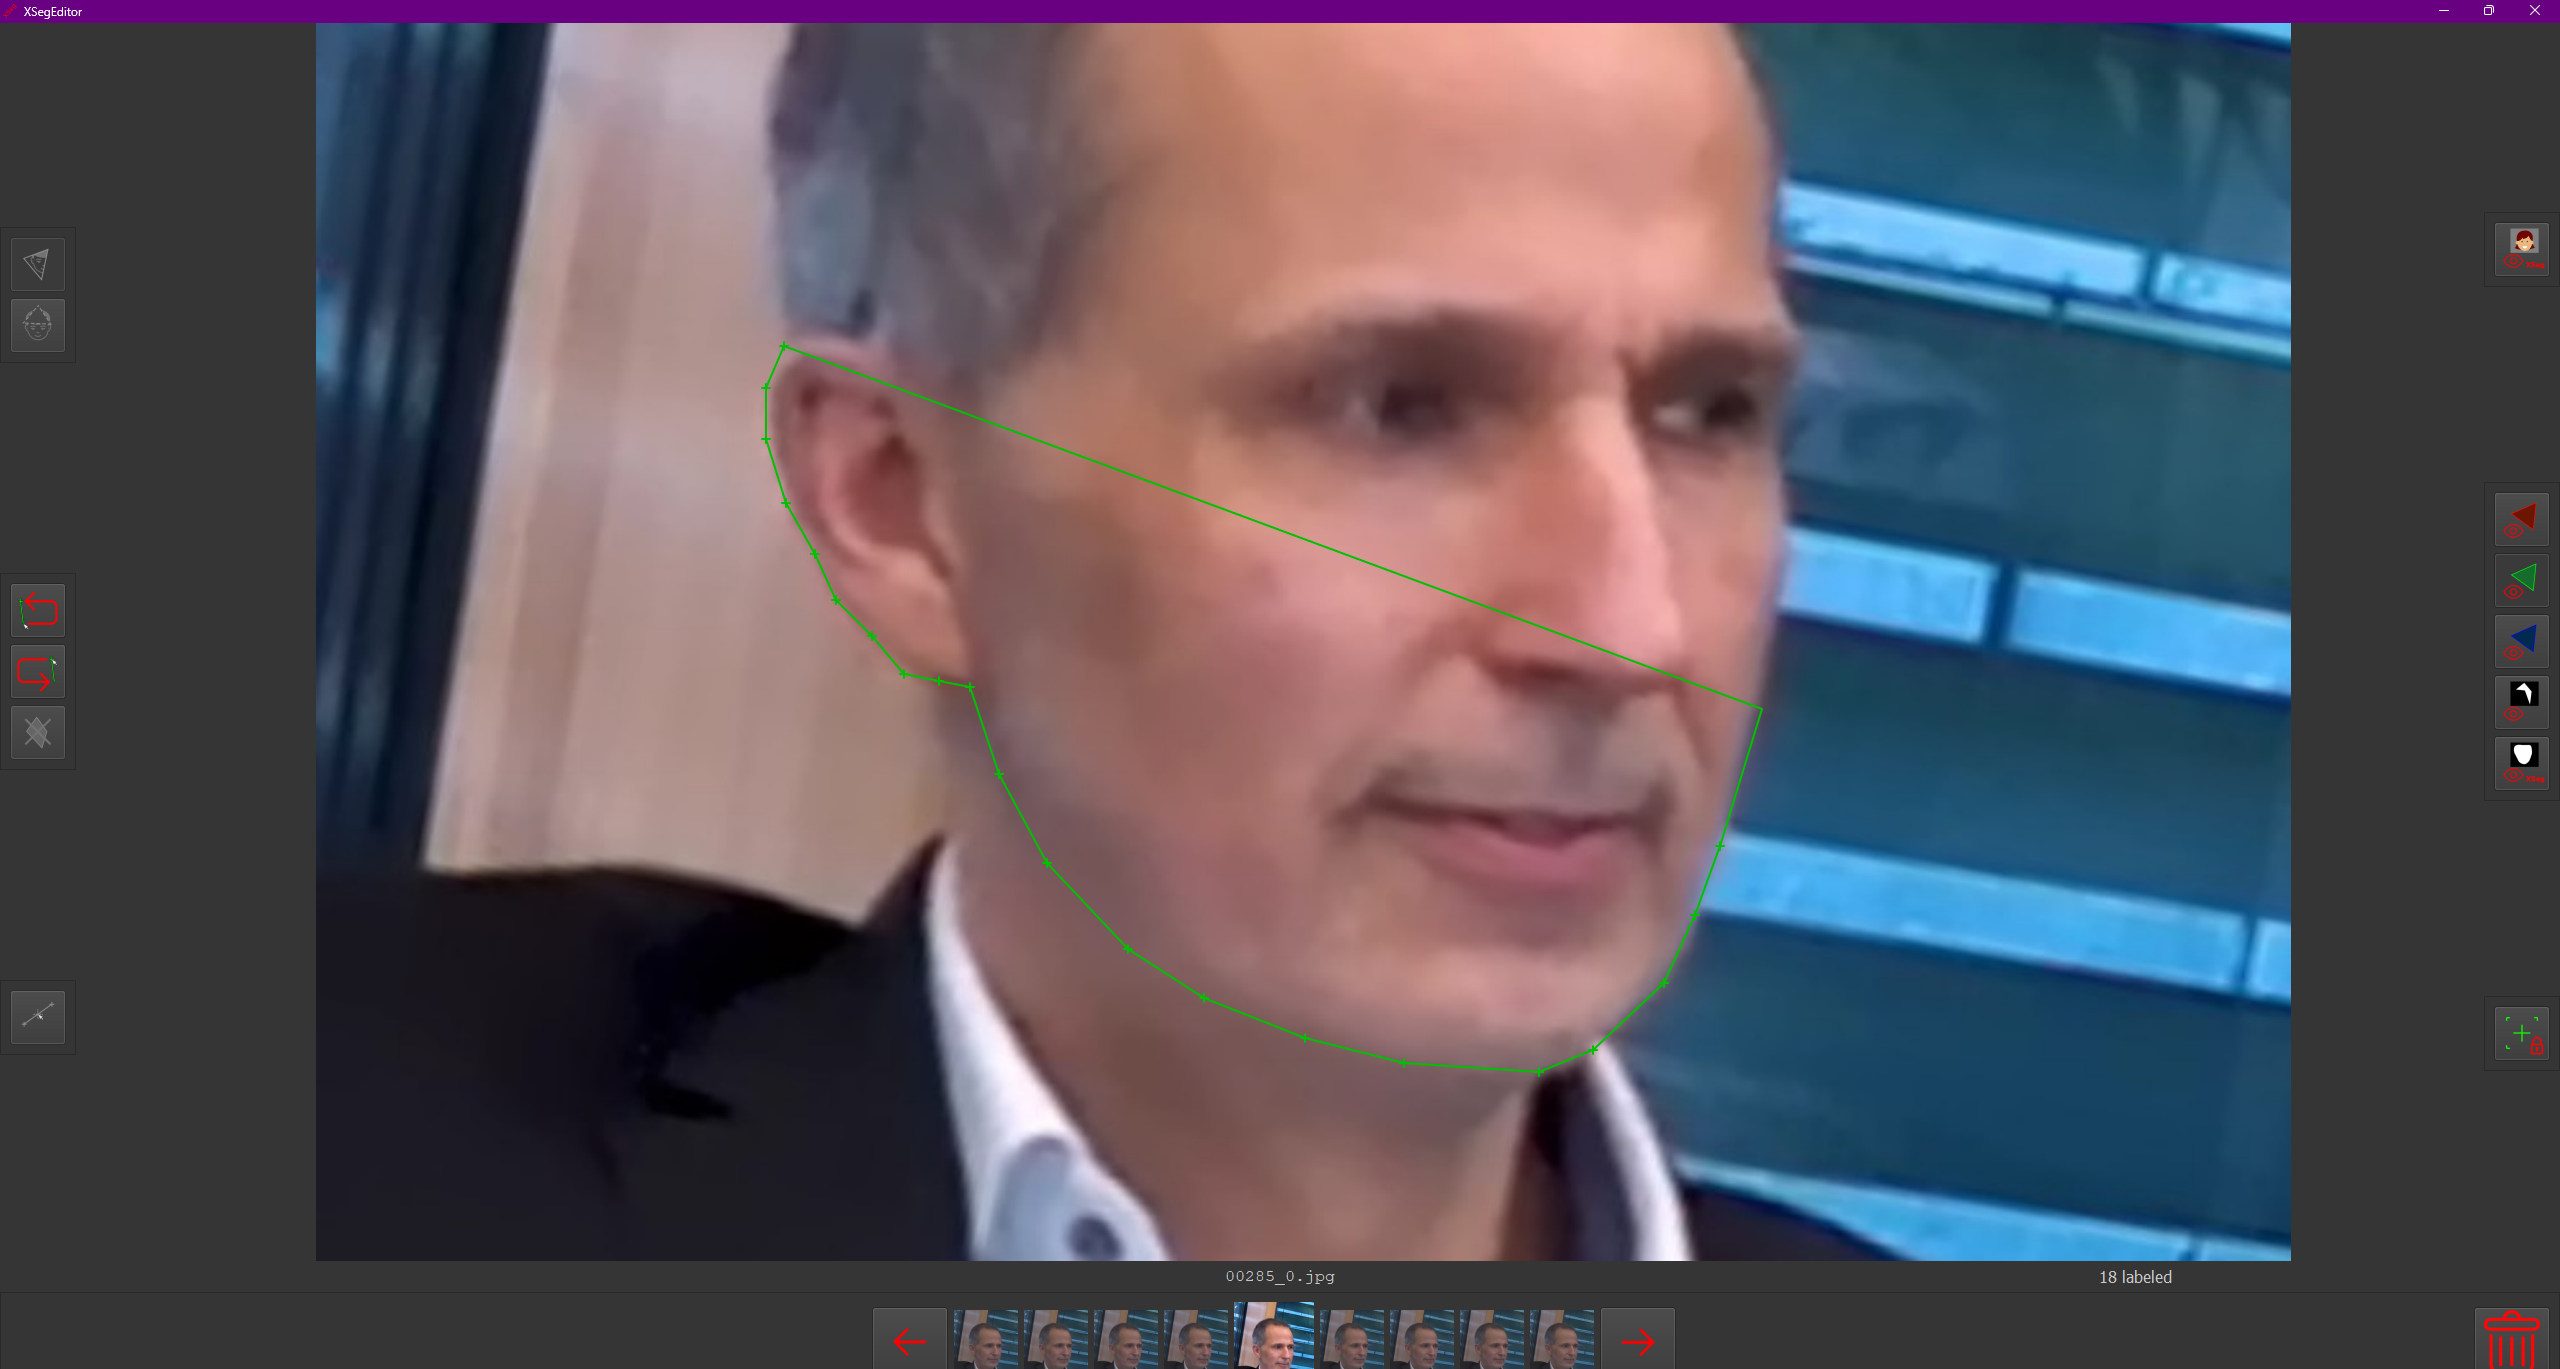
\includegraphics[width=0.7\textwidth]{Bilder/DFL/XSegEditor-1-draw}
    \caption{Polygon zeichnen im XSeg-Editor}
    \label{fig:xseg-editor-1}
\end{figure}
Es sollten je nach gewünschter Genauigkeit mehrere Dutzend bis wenige hundert Bilder markiert werden.
Dabei ist es entscheidend, möglichst viele verschiedene Ausdrücke und Kopfstellungen zu markieren und die Größe der Markierung konsistent zu halten.
Z.B. sollte die Kieferkontur immer gleich gezeichnet werden oder die Menge der Stirn, die maskiert werden soll.
Wurde der Prozess für \texttt{src} und \texttt{dst} durchgeführt, können die markierten Bilder in einen anderen Ordner verschoben werden und die Maske trainiert werden. Dabei werden die maskierten Bilder verwendet und zusätzlich automatisch verzerrt und eingefärbt (Abbildung \ref{fig:xseg-train}).
\begin{lstlisting}[label={lst:extraction-7},numbers=none]
    5.XSeg) data_src mask - fetch.bat
    5.XSeg) data_dst mask - fetch.bat
    5.XSeg) train.bat
\end{lstlisting}
\begin{figure}
    \center
    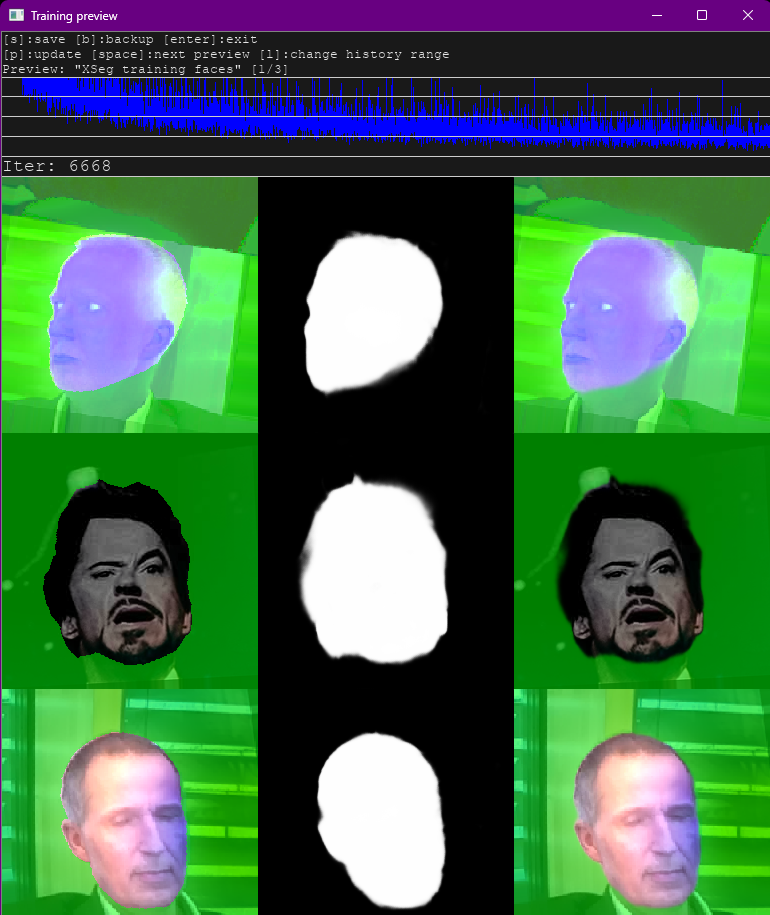
\includegraphics[width=0.7\textwidth]{Bilder/DFL/XSegEditor-4-train-1}
    \caption{Training von XSeg im \textit{head} Modus}
    \label{fig:xseg-train}
\end{figure}

Das Training sollte so lange fortgesetzt werden, bis die Konturen der Gesichter klar erkennbar sind.
Dies sollte i.d.R. nach einigen Tausend Iterationen der Fall sein (Abbild \ref{fig:xseg-train-result}).

\begin{figure}
    \center
    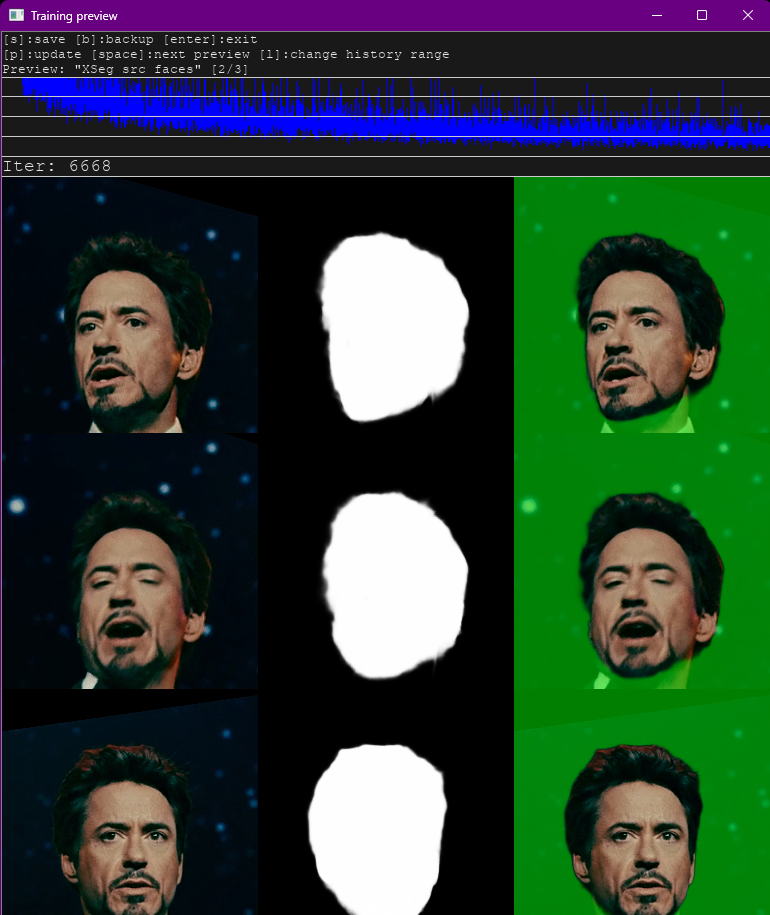
\includegraphics[width=0.7\textwidth]{Bilder/DFL/XSegEditor-4-train-3}
    \caption{Training Ergebnis von XSeg im \textit{head} Modus}
    \label{fig:xseg-train-result}
\end{figure}

Anschließend muss die trainierte Maske auf \texttt{src} und \texttt{dst} angewandt werden.
\begin{lstlisting}[numbers=none,label={lst:xseg-apply}]
    5.XSeg) data_src trained mask - apply.bat
    5.XSeg) data_dst trained mask - apply.bat
\end{lstlisting}
Danach kann die trainierte Maske im XSeg-Editor überprüft werden (Abbildung \ref{fig:xseg-train-comparison}).
Falls die Maske an manchen Stellen noch nicht passt, sollten diese Frames manuell markiert werden und danach das Training fortgeführt werden.
Anschließend muss die Maske neu angewandt werden.

\begin{figure}
    \center
    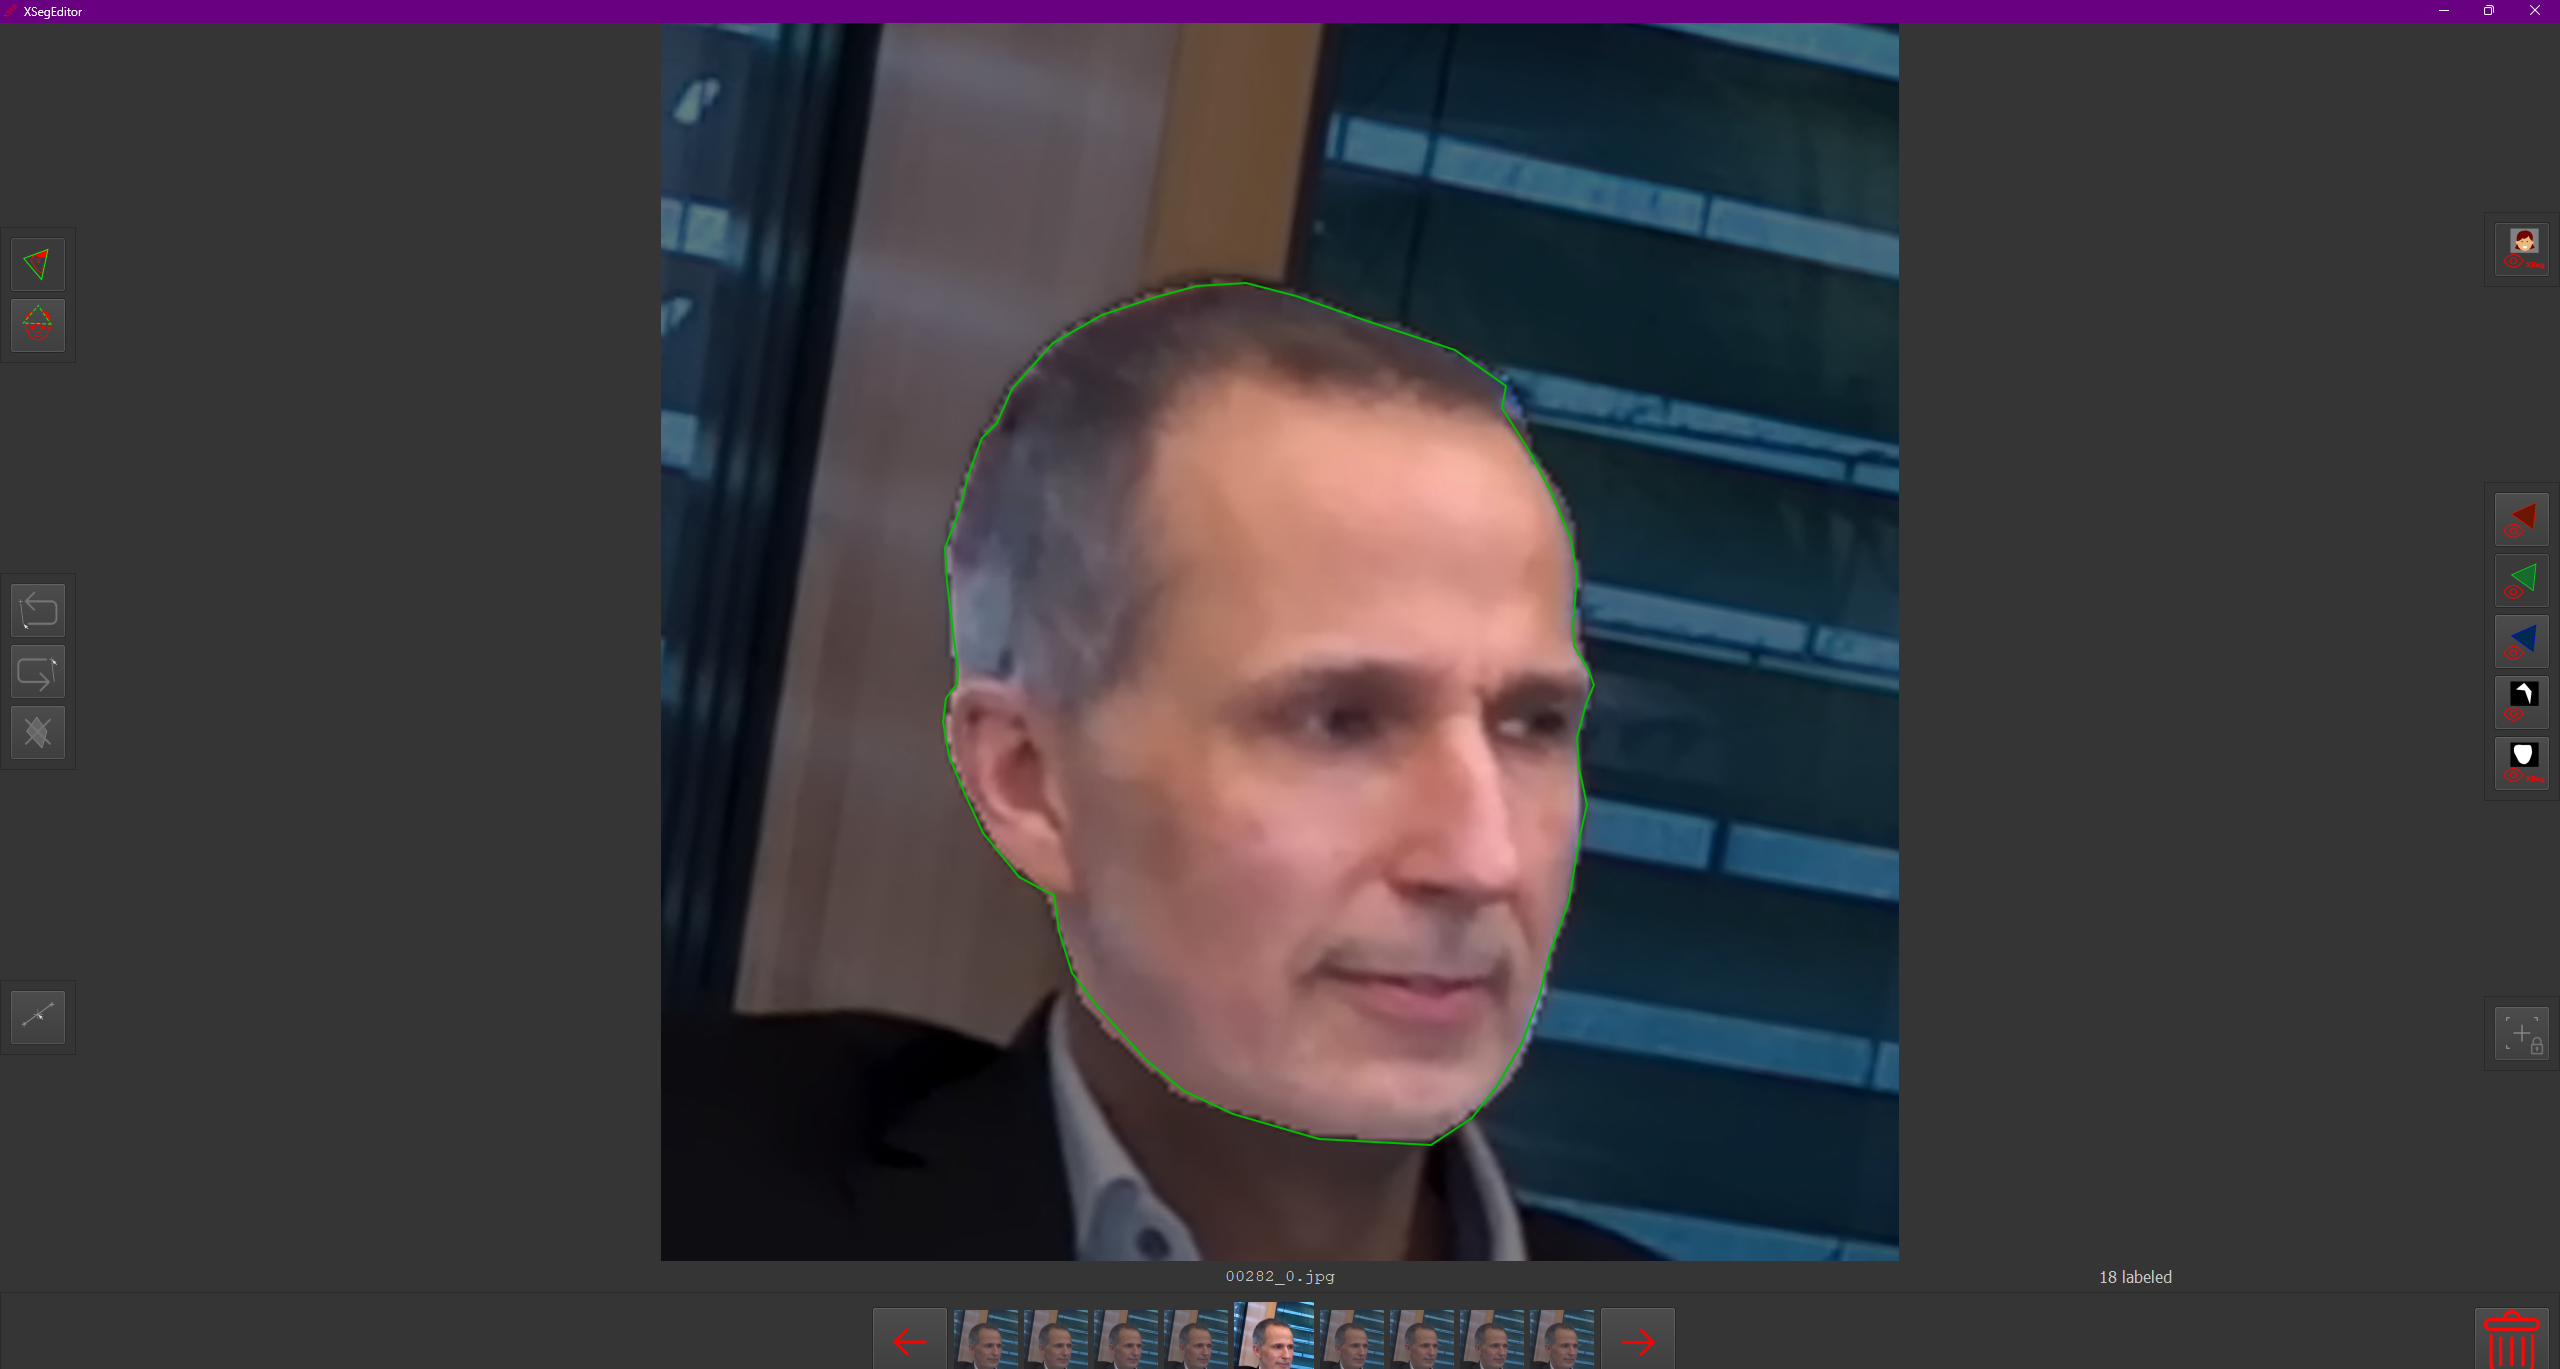
\includegraphics[width=0.7\textwidth]{Bilder/DFL/XSegEditor-6-trained-draw-comparision}
    \caption{Vergleich: Angewandtes XSeg-Model (highlight) und manuelle Markierung (grün)}
    \label{fig:xseg-train-comparison}
\end{figure}

\subsubsection{Facepack Erstellung}
Der letzte (optionale) Schritt der Extraktionsphase ist das Erstellen eines Facepacks.
Dies ist eine komprimierte Version der bisher geleisteten Arbeit.
Die bisherigen Schritte erforderten vergleichsweise wenig Rechenleistung; durch Facepacks lassen sich die Daten einfacher auf z.B. einen stärkeren Computer übermitteln.
\gls{dfl} speichert alle Informationen in den Bilddateien, daher könnten die Bilder auch einfach in einem Archiv verschickt werden.
Eine \texttt{.pak}-Datei ist allerdings der von \gls{dfl} bevorzugte Weg.
Ein Facepack beinhaltet immer nur die Informationen zu einem Gesicht, nicht einem Gesichterpaar.
Es müssen also zwei Pakete erstellt werden.
\begin{lstlisting}[numbers=none,label={lst:facepack}]
    4.2) data_src util faceset pack.bat
    5.2) data_dst util faceset pack.bat
\end{lstlisting}
